%\documentclass[xcolor=dvipsnames,9pt]{beamer} 
%\documentclass[xcolor=dvipsnames,9pt,hide notes,mathserif]{beamer}
\documentclass[xcolor=dvipsnames,9pt,handout,hide notes,mathserif]{beamer}

\usepackage{pgfpages}
\usepackage{listings}
%\usepackage{enumitem}

%% For creating a handout:
\pgfpagesuselayout{4 on 1}[border shrink=5mm]
%\pgfpagesuselayout{4 on 1}[landscape, border shrink=5mm]
\pgfpageslogicalpageoptions{1}{border code=\pgfusepath{stroke}}
\pgfpageslogicalpageoptions{2}{border code=\pgfusepath{stroke}}
\pgfpageslogicalpageoptions{3}{border code=\pgfusepath{stroke}}
\pgfpageslogicalpageoptions{4}{border code=\pgfusepath{stroke}}
%\mode<handout>{\setbeamercolor{background canvas}{bg=black!5}}

%% For creating notes for the speaker:
%\setbeameroption{notes on second screen}
%\setbeameroption{show notes}

\setbeamerfont{structure}{family=\rmfamily,shape=\scshape} 
\usepackage{graphicx}
\usepackage{tikz}
\usepackage{scalefnt}
\usepackage{amsmath}%
\usepackage{amsfonts}%
\usepackage{amssymb}%
%(wjd) added stmaryrd and enumerate packages
\usepackage{stmaryrd,enumerate}
\usepackage{graphicx}
\usepackage{comment}
\usetikzlibrary{matrix,arrows}

\usepackage{mathrsfs,textcomp}
\setbeamertemplate{navigation symbols}{}
\usepackage{verbatim}
\usepackage[mathcal]{euscript}

% This changes the color of alerted text to blue:
\definecolor{MyDarkBlue}{rgb}{0.2,0.2,0.7}
\definecolor{olivegreen}{cmyk}{0.64,0,0.95,0.40} % PANTONE 582
\setbeamercolor{alerted text}{fg=blue}
\newcommand{\emphcyan}[1]{\textcolor{MyDarkBlue}{\textbf{#1}}}
%\renewcommand{\alert}[1]{\textcolor{olivegreen}{\emph{#1}}}
\renewcommand{\alert}[1]{\textcolor{olivegreen}{#1}}
%\renewcommand{\alert}[1]{\textbf{{\emph{#1}}}}
% (default is red, but my slides are green and I don't like red and green together)

%\usecolortheme[named=OliveGreen]{structure} 
\usecolortheme[named=olivegreen]{structure} 
\setbeamertemplate{items}[square] 
\setbeamertemplate{blocks}[rounded][shadow=false]


%%
%% This is file `wjd.def'
%%
%%% ====================================================================
%%% @LaTeX-file{
%%%   filename  = "wjd.def",
%%%   version   = "0.03.09.08",
%%%   date      = "2003/09/08",
%%%   author    = "William DeMeo",
%%%   email     = "williamdemeo@yahoo.com"
%%% }
%%% ====================================================================
%% 
% -------------------------------------------------------------
% Custom Math Definitions 
% -------------------------------------
%  Algebra & Analysis:
   \newcommand{\field}[1]{\ensuremath{\mathbb{#1}}}
   \newcommand{\Z}{\field{Z}}                   % integers
   \newcommand{\Q}{\field{Q}}                   % rational numbers
   \newcommand{\N}{\field{N}}                   % natural numbers
   \def\R{\field{R}}                   % real numbers 
   \newcommand{\Rn}{\ensuremath{\field{R}^n}}                % the set of n-tuples with elements in \R
   \newcommand{\C}{\field{C}}                   % complex numbers 
   \newcommand{\Cn}{\ensuremath{\field{C}^n}}                % the set of n-tuples with elements in \C
   \newcommand{\rel}{\ensuremath{\mathcal{R}}}                % a general relation
   \newcommand{\Gplus}{\ensuremath{\langle G, + \rangle}}  % a group with binary op \cdot
   \newcommand{\Gdot}{\ensuremath{\langle G, \cdot \rangle}}   % a group with binary op \cdot
   \newcommand{\Group}{\ensuremath{\langle G, * \rangle}}      % a group with binary op *
   \newcommand{\Ring}{\ensuremath{\langle R, +, \cdot \rangle}} % a ring
   \newcommand{\F}{\field{F}}                   % a field
   \newcommand{\Fn}{\ensuremath{\field{F}^n}}                % the set of n-tuples with elements in \F
   \newcommand{\FN}{\ensuremath{\field{F}^N}}                % the set of N-tuples with elements in \F
   \newcommand{\ztwo}{\ensuremath{\field{Z}_2}}              % Cyclic groups (rings)
   \newcommand{\zthree}{\ensuremath{\field{Z}_3}}
   \newcommand{\zfour}{\ensuremath{\field{Z}_4}}
   \newcommand{\Real}{\mbox{Re}} % real part of a complex number  ALT: \newcommand{\Real{\Re}
   \newcommand{\Imag}{\mbox{Im}}
   \newcommand{\integral}{\ensuremath{\int_{-\infty}^{\infty}}}% integration ALT: \newcommand{\integral{\int_{-\infty}^{+\infty}} 

%  Operator Theory and Vector Spaces
   \newcommand{\pv}{\ensuremath{\operatorname{pv}}}
   \newcommand{\W}{\ensuremath{\operatorname{W}}}       % an operator (\eg Wigner-Ville transform)
   \newcommand{\Per}{\ensuremath{\operatorname{Per}}}   % a periodizing operator

   %linear transformations \lt should be sans-serif
   \newcommand{\lt}[1]{\ensuremath{\mathsf{#1}}}
   \newcommand{\ltb}[1]{\ensuremath{[\mathsf{#1}]}}
   \newcommand{\linmap}[3]{\ensuremath{\lt{#1}: \vs{#2} \rightarrow \vs{#3}}}
   \renewcommand{\S}{\lt{S}}       % a linear operator (\eg translation)
   \newcommand{\T}{\lt{T}}       % a linear operator (\eg translation)
   \newcommand{\eye}{\lt{I}}     % the identity operator
   \newcommand{\eyeb}{[\,\lt{I}\,]}     % the identity operator

   % vector spaces should appear in mathcal font.
   \newcommand{\vs}[1]{\ensuremath{\mathcal{#1}}}
   \newcommand{\Lp}{\ensuremath{L^p}}%\newcommand{\Lone}{\vs{L}^1}
   \newcommand{\Linfty}{\ensuremath{L^\infty}}%\newcommand{\Lone}{\vs{L}^1}
   \newcommand{\Lone}{\ensuremath{L^1}}%\newcommand{\Lone}{\vs{L}^1}
   \newcommand{\Ltwo}{\ensuremath{L^2}}%\newcommand{\Ltwo}{\vs{L}^2}
   \newcommand{\ltwo}{\ensuremath{\ell^2}}
   \newcommand{\LpR}{\Lp(\R)}
   \newcommand{\LoneR}{\Lone(\R)}
   \newcommand{\LtwoR}{\Ltwo(\R)}
   \newcommand{\ltwoR}{\ltwo(\R)}
   \newcommand{\LA}{\vs{L}(A)}        % the collection of complex valued functions of $A$.
   \newcommand{\LG}{\vs{L}(G)}        % the collection of complex valued functions of $G$.
   \newcommand{\LZN}{\vs{L}(\Z/N)}    % the collection of complex valued functions of $\Z/N$.
   \newcommand{\Hilbert}{\vs{H}}      % a Hilbert space
   \newcommand{\Banach}{\vs{B}}       % a Banach space
   %   \newcommand{\BanachHH}{\Banach(\Hilbert,\Hilbert)}   % a Banach space
   \newcommand{\Hone}{\vs{H}_1}
   \newcommand{\Htwo}{\vs{H}_2}
   %   \newcommand{\BanachHoneHtwo}{\vs{B}(\Hone,\Htwo)}}
   %   \newcommand{\BanachHtwoHone}{\vs{B}(\Htwo,\Hone)}}
   \newcommand{\esssup}[1]{\ensuremath{\text{ess}\sup_{#1}}}

% old:   
%   \newcommand{\T}{\ensuremath{\operatorname{T}}}
%   \newcommand{\Hilbert}{\ensuremath{\mathcal{H}}}      % a Hilbert space
%   \newcommand{\Hone}{\ensuremath{\mathcal{H}_1}}
%   \newcommand{\Htwo}{\ensuremath{\mathcal{H}_2}}
%   \newcommand{\Banach}{\ensuremath{\mathcal{B}(\Hilbert,\Hilbert)}}   % a Banach space
%   \newcommand{\Banachonetwo}{\ensuremath{\mathcal{B}(\Hone,\Htwo)}}
%   \newcommand{\Banachtwoone}{\ensuremath{\mathcal{B}(\Htwo,\Hone)}}


   \newcommand{\ga}[1]{\ensuremath{\C #1}} %  group algebras
   \newcommand{\CA}{\ga{A}}                % the group algebra of $A$
   \newcommand{\CG}{\ga{G}}                % the group algebra of $G$
   \newcommand{\basis}{\ensuremath{\mathcal{B}}}     % basis
   \newcommand{\Span}{\ensuremath{\mbox{span}}}
   \newcommand{\Null}{\ensuremath{\mathcal{N}}}      % null space
   \newcommand{\Range}{\ensuremath{\mathcal{R}}}     % range
   \newcommand{\Krylov}{\ensuremath{\mathcal{K}}}    
   \newcommand{\FT}{\ensuremath{\mathcal{F}}}    % fourier transform
   \newcommand{\invFT}{\ensuremath{\mathcal{F}^{-1}}} % inverse fourier transform
   \newcommand{\Poi}{\ensuremath{\operatorname{Poi}}}   % Poisson distribution

% The following definition was for manual bolding of vectors:
%   \newcommand{\bx}{\ensuremath{\mathbf{x}}}
% It is ugly and deprecated; better to use the \vec command; e.g. \vec{x}  
%   @ifundefined{vec}{\newcommand{\vec}[1]{\mathbf{#1}}}{}
%   \newcommand{\vec}[1]{\mathbf{#1}}

   \newcommand{\mean}[1]{\overline{#1}} % sample mean of x
% should now use \mean{x} instead of:
%   \newcommand{\sm}{\ensuremath{\overline{x}}}    % sample mean of x
   \newcommand{\Prob}{\field{P}}                      % a probability distribution

% Latin (see LaTeX Companion, p. 50)
   \newcommand{\eg}{e.g.,\space}            % for example (latin: {\it exempli gratia})
   \newcommand{\ie}{i.e.,\space}            % that is     (latin: {\it id est})
   \newcommand{\etc}{etc.\@\space}          % etcetera    (latin: {\it et cetera})
\newcommand{\dotcup}{\ensuremath{\mathaccent\cdot\cup}}

\newcommand\defeq{\ensuremath{\stackrel{\text{def}}{=}}}
\newcommand\net{\ensuremath{\{x_\alpha\}}}
\newcommand\Net{\ensuremath{\{x_\alpha : \alpha \in A\}}}
\newcommand\Netn{\ensuremath{\{x_\alpha : \alpha \in A_n\}}}
\newcommand\rsum{\ensuremath{R(f,P,c)}}
\newcommand\intab{\ensuremath{\int_a^b}}
\newcommand\unsolved{\textcolor{red}{\it Have yet to solve this one!}}
\newcommand\onlyif{\ensuremath{\quad \Rightarrow \quad}}
\newcommand\iif{\ensuremath{\quad \Leftrightarrow \quad}}

\newcommand{\inverse}[1]{\ensuremath{#1^{-1}}}
\newcommand{\inv}[1]{\ensuremath{#1^{-1}}}
\newcommand{\transpose}[1]{\ensuremath{#1^{\lt{t}}}}
\newcommand{\compl}[1]{\ensuremath{#1^{\complement}}}
\newcommand{\smallfrac}[2]{\ensuremath{{\scriptstyle \frac{#1}{#2}}}}
\newcommand{\Clifford}[2]{\ensuremath{\mathcal{C\ell}_{#1,#2}}}

% Memorandum meta data fields
\newcommand{\memometa}[2]{\underline{{\sc {\bf #1:}}}\; #2\\\\}
\newcommand{\memohead}[1]{\lhead{{\sc Textron} Systems}\chead{{\sc Memorandum}}\rhead{#1}}
%\newcommand{\memosec}[1]{\noindent\underline{\bf #1}}
\newcommand{\memosec}[1]{\begin{center}\noindent {\bf #1}\end{center}}

\newcommand{\given}{\ensuremath{\,|\,}}
%\newcommand{\indicator}[1]{\ensuremath{\vec{1}(#1)}}
\newcommand{\vA}{\ensuremath{\vec{A}}}
\newcommand{\vU}{\ensuremath{\vec{U}}}
\newcommand{\Uperp}{\ensuremath{\vec{U}_\perp}}
\newcommand{\Upara}{\ensuremath{\vec{U}_\parallel}}
\newcommand{\Uparaa}{\ensuremath{\vec{U}_{\va}}}
\newcommand{\uperp}{\ensuremath{\vec{u}_\perp}}
\newcommand{\upara}{\ensuremath{\vec{u}_\parallel}}
\newcommand{\vperp}{\ensuremath{\vec{v}_\perp}}
\newcommand{\vpara}{\ensuremath{\vec{v}_\parallel}}

\newcommand\eone{\ensuremath{\vec{e}_1}}
\newcommand\etwo{\ensuremath{\vec{e}_2}}
\newcommand\ethree{\ensuremath{\vec{e}_3}}
\newcommand\Itwo{\ensuremath{\vec{I}_2}}
\newcommand\ITWO{\ensuremath{\eone \wedge \etwo}}
\newcommand\Ithree{\ensuremath{\vec{I}_3}}
\newcommand\ITHREE{\ensuremath{\eone \wedge \etwo \wedge \ethree}}
\newcommand\carrot{\ensuremath{\wedge}}
\newcommand\dual{\text{dual}}
\newcommand\va{\ensuremath{\vec{a}}}
\newcommand\vb{\ensuremath{\vec{b}}}
\newcommand\vB{\ensuremath{\vec{B}}}
\newcommand\vc{\ensuremath{\vec{c}}}
\newcommand\vY{\ensuremath{\vec{Y}}}
\newcommand\vw{\ensuremath{\vec{x}}}
\newcommand\vu{\ensuremath{\vec{u}}}
\newcommand\vv{\ensuremath{\vec{v}}}
\newcommand\vx{\ensuremath{\vec{x}}}
\newcommand\vy{\ensuremath{\vec{y}}}
\newcommand\vz{\ensuremath{\vec{z}}}
\newcommand\indicator[1]{\ensuremath{\vec{1}\{#1\}}}

% might use \startcodebox{12}
\newcommand{\startcodebox}[1]{\begin{center}\setlength{\fboxsep}{4mm}\begin{boxedminipage}[t]{#1cm}}
\newcommand\stopcodebox{\end{boxedminipage}\end{center}\vspace{2mm}}

%--- begin 2004.11.01 additions ---
%\newcommand\UCB{U.~C.~Berkeley}
\newcommand{\school}[1]{{\large{\itshape{#1}}}}
\newcommand{\inst}[1]{{\large{\itshape{#1}}}}
\newcommand{\job}[1]{{\small{\bfseries\sffamily{#1}}}}
\newcommand\hsptwo{}
\newcommand\adjsl{\small  \vspace*{-10pt}}  
\newcommand\brr{\begin{raggedright}}
\newcommand\err{\end{raggedright}}
\newcommand\smallsep{\setlength{\itemsep}{-1pt}}
\newcommand\bigsep{\setlength{\itemsep}{+1pt}}
\newcommand\Yj{\ensuremath{Y_j}}
\newcommand\Xij{\ensuremath{X(i,j)}}
\newcommand{\bi}{\begin{itemize}} 
\newcommand{\ei}{\end{itemize}} 
\newcommand{\bis}{\begin{itemstep}} 
\newcommand{\eis}{\end{itemstep}} 
\newcommand\yields{\ensuremath{\leadsto \;}} 
%--- end 2004.11.01 additions ---

\newcommand\e{\mathrm{e}}    % exponential
   \newcommand\A{\operatorname{A}}
%   \newcommand\E{\operatorname{E}}   % prefer to use \E for e = 3.14...
   \renewcommand\H{\operatorname{H}}
%   \newcommand\I{\operatorname{I}}   % prefer to use \I for imaginary number
   \newcommand\Banachonetwo{\mathcal{B}(\Hone,\Htwo)}
   \newcommand\Banachtwoone{\mathcal{B}(\Htwo,\Hone)}
% Signals, Time-Frequency shifts, etc.
   \newcommand\scale{\frac{1}{\sqrt{s}}}
   \newcommand\transcale{\left(\frac{t-u}{s}\right)}
   \newcommand\xpull{x_{\frac{\tau}{2}, -\frac{\xi}{2}}}
   \newcommand\xpush{x_{-\frac{\tau}{2}, \frac{\xi}{2}}}
   \newcommand\xpullpush{x_{\frac{\tau}{2}, \frac{\xi}{2}}}
   \newcommand\xpushpull{x_{-\frac{\tau}{2}, -\frac{\xi}{2}}}
   \newcommand\xfpull{x_{-\frac{\Delta\nu}{2}}}
   \newcommand\xfpush{x_{\frac{\Delta\nu}{2}}}
   \newcommand\apull{a_{-}}
   \newcommand\apush{a_{+}}
   \newcommand\ytnu{y_{t,\nu}}
   \newcommand\ytnut{\tilde{y}_{t,\nu}}
   \newcommand\half{{\scriptstyle \frac{1}{2}}}
   \newcommand\halftau{{\scriptstyle \frac{\tau}{2}}}
   \newcommand\halfxi{{\scriptstyle \frac{\xi}{2}}}
   \newcommand\halfnu{{\scriptstyle \frac{\nu}{2}}}
   \newcommand\halfDnu{{\scriptstyle \frac{\Delta\nu}{2}}}
   \newcommand\xtpull{x\left(t+\halftau\right)}
   \newcommand\xtpush{x\left(t-\halftau\right)}
%   (shouldn't need this) \newcommand\xtpullconj{x^*\left(t+\halftau\right)}
   \newcommand\xtpushconj{x^*\left(t-\halftau\right)}
   \newcommand\Xtpull{X\left(\nu+\halfxi\right)}
   \newcommand\Xtpush{X\left(\nu-\halfxi\right)}
   \newcommand\Xtpullconj{X^*\left(\nu+\halfxi\right)}
%   (shouldn't need this) \newcommand\Xtpushconj{X^*\left(\nu-\halfxi\right)}

   \newcommand\ytpull{y\left(t+\halftau\right)}
   \newcommand\ytpush{y\left(t-\halftau\right)}
%   (shouldn't need this) \newcommand\ytpullconj{y^*\left(t+\halftau\right)}
   \newcommand\ytpushconj{y^*\left(t-\halftau\right)}
   \newcommand\Ytpull{Y\left(\nu+\halfxi\right)}
   \newcommand\Ytpush{Y\left(\nu-\halfxi\right)}
   \newcommand\Ytpullconj{Y^*\left(\nu+\halfxi\right)}
%   (shouldn't need this) \newcommand\Ytpushconj{Y^*\left(\nu-\halfxi\right)}

% Language
%   \newcommand\FT{Fourier transform}
   \newcommand\WT{Wigner transform}
   \newcommand\WV{Wigner-Ville}


%% Customized section style commands

   \newcommand{\wjdsecstyle}{\scshape\boldmath}
   \newcommand{\wjdsubsecstyle}{\scshape\boldmath}

%     \newcommand\wjdsec[1]{\chapter{\normalfont\wjdsecstyle #1}}
%     \newcommand\wjdsec[1]{\chapter{#1}}
     \newcommand\wjdsec[1]{\section{#1}}
     \newcommand\wjdsubsec[1]{\subsection{#1}}
     \newcommand\wjdsubsubsec[1]{\subsubsection{#1}}
%     \newcommand\wjdparasec[1]{\paragraph{#1}}
     \newcommand\wjdparasec[1]{\subsubsection{#1}}
     \newcommand\wjdappsec[1]{\section{#1}}
     \newcommand\wjdappsubsec[1]{\subsection{#1}}
%     \newcommand\wjdappsubsubsec[1]{\paragraph{#1}}
     \newcommand\wjdappsubsubsec[1]{\subsubsection{#1}}
%     \newcommand\wjdappparasec[1]{\subparagraph{#1}}
     \newcommand\wjdappparasec[1]{\subsubsection{#1}}

     \newcommand\hafgsec[1]{\section{#1}}
     \newcommand\hafgsubsec[1]{\subsection{#1}}
     \newcommand\hafgsubsubsec[1]{\subsubsection{#1}}
     \newcommand\hafgparasec[1]{\paragraph{#1}}

   \newcommand\ismasec[1]{\section{#1}}
   \newcommand\ismasubsec[1]{\subsection{#1}}
   \newcommand\ismasubsubsec[1]{\subsubsection{#1}}
   \newcommand\ismaparasec[1]{\subsubsection{#1}}


   % Binary operator symbols
   \newcommand\sdp{\ensuremath{\varangle}}                      % semi-direct product

   \newcommand\scriptfrac[2]{\ensuremath{{\scriptstyle \frac{#1}{#2}}}}

\newcommand{\functionsec}[1]{\wjdparasec{\hrule\vspace{1mm}\noindent#1}}
\newcommand{\rootxref}[1]{The main function definition begins
  at $\langle${\it #1} \subpageref{root:#1}$\rangle$.}
\newcommand{\shortrootxref}[1]{The main function definition begins
  at chunk~\subpageref{root:#1}.}

\newcommand{\authorref}[1]{{\scshape #1}}

\newcommand{\dotB}{\ensuremath{\dot{\vec{B}}}}
\newcommand{\dotH}{\ensuremath{\dot{\vec{H}}}}
\newcommand{\dotE}{\ensuremath{\dot{\vec{E}}}}
\newcommand{\DdotE}{\ensuremath{\Ddot{\vec{E}}}}
\newcommand{\dotD}{\ensuremath{\dot{\vec{D}}}}
\newcommand{\DdotD}{\ensuremath{\Ddot{\vec{D}}}}

\newcommand{\curl}{\ensuremath{\mathrm{curl\,}}}
\renewcommand{\div}{\ensuremath{\mathrm{div\,}}}
\newcommand{\grad}{\ensuremath{\mathrm{grad\,}}}

% Special notation for exponents and the imaginary number
\newcommand{\E}{\ensuremath{\mathrm{e}}}
\newcommand{\I}{\ensuremath{\mathrm{i}}}

%
% --- Radar and Imaging Definitions ---
%
\newcommand\autocorrelation{\ensuremath{\hat{R}_{\hat{f}\hat{f}}}}
\newcommand\MIf{\ensuremath{\hat{R}_{\hat{f}\hat{f}}}}
\newcommand{\MI}[1]{\ensuremath{\hat{R}_{\hat{#1}\hat{#1}}}}
\newcommand\Pupil{\ensuremath{\vs{P}}}
\newcommand\Focal{\ensuremath{\vs{F}}}
%\newcommand\micro{\ensuremath{\mu}}
\newcommand{\micro}[1]{\ensuremath{\mu\text{#1}}}
\newcommand\km{\ensuremath{\text{km}}}
\newcommand\nmi{\ensuremath{\text{nmi}}}
%\newcommand\Tintrapulse{\ensuremath{\tau_{\text{intrapulse}}}}
\newcommand\pbw{\ensuremath{\tau_{\text{b}}}}  % pulse-burst width
\newcommand\ptw{\ensuremath{\tau_{\text{t}}}}  % pulse-tone width
\newcommand\prp{\ensuremath{T_{\text{p}}}}  % pulse repetition period
\newcommand\prf{\ensuremath{f_{\text{p}}}}  % pulse repetition frequency

\newcommand{\zmv}{\ensuremath{x^m k_v}}
\newcommand{\zmvInv}{\ensuremath{x^{N-wm} k_w}}


% [NB Include file 'wjdthms.def' for end-of-proof symbol]
%\newcommand\qedsymbol{\hbox{\rlap{$\sqcap$}$\sqcup$}}
%\newcommand\qed{\relax\ifmmode\else\unskip\quad\fi\qedsymbol}
%\newcommand\smartqed{\renewcommand\qed{\relax\ifmmode\qedsymbol\else
%  {\unskip\nobreak\hfil\penalty50\hskip1em\null\nobreak\hfil\qedsymbol
%  \parfillskip=\z@\finalhyphendemerits=0\endgraf}\fi}}

%\smartqed

%%-------------------------------------------------------------


\mode<presentation>{\usetheme{boxes}}  %boxes,Pittsburgh JuanLesPins, PaloAlto, Singapore, Szeged, Warsaw, Boadilla
%\usetheme{Madrid}}
%\usetheme{boxes}  %boxes,Pittsburgh JuanLesPins, PaloAlto, Singapore, Szeged, Warsaw, Boadilla

\usepackage[english]{babel}
\usepackage[latin1]{inputenc}
\usepackage{times}
\usepackage[T1]{fontenc}
% Or whatever. Note that the encoding and the font should match. If T1
% does not look nice, try deleting the line with the fontenc.

\title{The Algebraic Approach to CSP\\
{\small and}\\
CSPs of Commutative Idempotent Binars}

\author[William DeMeo]{William DeMeo\\
  {\small \url{williamdemeo@gmail.com}}\\[4pt]
%  {\small Iowa State University}\\[4pt]
  {\footnotesize joint work with}\\[4pt] 
  Cliff Bergman\\
  Jiali Li
}
\institute{Iowa State University}

\date[BLAST 2015]{ % (optional, should be abbreviation of conference name)
  BLAST 2015\\{\small University of North Texas}\\
  {\small June 8--12}}

\subject{Universal Algebra; Lattice Theory; CSP.}% (optional) inserted into PDF info catalog.

\begin{document}
\thicklines

\includeonlyframes{titlepage,intro,intro2,intro3,intro4,intro5,intro6,problem1,cib,general1,cube,cp,general2,remaining,examples1,examples2,examples3,examples4,others}
%%\includeonlyframes{intro6}


\frame[label=titlepage]{
  \titlepage
  \hfill {\footnotesize slides available at\\ 
\hfill \url{https://github.com/williamdemeo/Talks}}
}


%%%%%%%%%%%%%%%%%%%%%%%%%%%%%%%%%%%%%%%%%%%%%%%%%%%%%%%%%%%
%% 1: CSP Intro 1
\frame[label=intro]{
  \frametitle{Constraint Satisfaction Problems}
%  \underline{Input}
  {\bf Input}
  \begin{itemize}
  \item \emph{variables:} $V = \{v_1, v_2, \dots\}$
  \item \emph{domain:}  $D$
  \item \emph{constraints:} $C_1, C_2, \dots$
  \end{itemize}
  \vskip1cm
%  \underline{Output}
 {\bf Output}
  \begin{itemize}
  \item ``yes'' if there is a \emph{solution}  
    \[
    \sigma : V \rightarrow D \quad 
    \text{    {\small (an assignment of values to variables that satisfies all $C_i$)}}
    \] 

  \item ``no'' otherwise
  \end{itemize}

}

\note{
  In computer science, the Boolean Satisfiability Problem 
  (abbreviated as SAT) is the problem of determining if there exists an
  \emph{interpretation} that satisfies a given Boolean formula. 

  In other words, it asks whether the \emph{variables} of a given Boolean
  formula can be consistently replaced by the values TRUE or FALSE in such a
  way that the formula evaluates to TRUE. 

  If this is the case, then the formula is called \emph{satisfiable}. 
  On the other hand, if no such assignment exists, the function expressed by
  the formula is identically FALSE for all possible variable assignments and
  the formula is unsatisfiable. For example, the formula ``$x \meet \neg y$'' is
  satisfiable because one can find the values, namely $x = 1$ and $y = 0$, 
  which make $(x \meet \neg y) = 1$. 

  In contrast, ``$x \meet \neg x$'' is unsatisfiable. 
}


%%%%%%%%%%%%%%%%%%%%%%%%%%%%%%%%%%%%%%%%%%%%%%%%%%%%%%%%%%%
%% 2: CSP intro 2
\frame[label=intro2]{
  \frametitle{Constraint Satisfaction Problems}
  \framesubtitle{Example: 3-SAT}
%  \underline{Input}
  {\bf Input}
  \begin{itemize}
  \item \emph{variables:} $V = \{v_1, \dots, v_n\}$
  \item \emph{domain:} $D = \{0, 1\}$
  \item \emph{constraints:} a formula, say,
    \[
    f(v_1, \dots, v_n) = (v_1 \join v_2 \join \neg v_3) \meet 
    (\neg v_1 \join v_3 \join v_4) \meet  \cdots
    \] 
  \end{itemize}
%  \underline{Output}
 {\bf Output}
  \begin{itemize}
  \item ``yes'' if there is a solution:  $\sigma : V \rightarrow D$ such that
    \[
    f(\sigma v_1,\dots, \sigma v_n) = 1
    \]
  \item ``no'' otherwise
  \end{itemize}
}

%%%%%%%%%%%%%%%%%%%%%%%%%%%%%%%%%%%%%%%%%%%%%%%%%%%%%%%%%%%
%% 3: CSP intro 3
\frame[label=intro3]{
  \frametitle{Constraint Satisfaction Problems}
  \framesubtitle{Example: NAE-SAT}
%  \underline{Input}
  {\bf Input}
  \begin{itemize}
  \item  \emph{variables:} $V = \{v_1, \dots, v_n\}$
  \item \emph{domain:} $D = \{0, 1\}$
  \item \emph{constraints:} $(s_1,C_1), (s_2,C_2),\dots $ {\small of the form}
    \begin{align*}
    s &= (i, j, k) \in \{1, \dots, n\}^3  \qquad \text{ {\small (scopes)}}\\
    C &= \neg (v_i = v_j = v_k)%  \qquad \text{ {\small (constraints)}}
    \end{align*}
    %% $(s_1,C_1), (s_2,C_2), \dots$ where 
    %% \begin{itemize}
    %% \item $s_i = (i_1, i_2, i_3) \in [n]^3$ {\small ``scopes''}
    %% \item $C_i = \neg (v_{i_1} = v_{i_2} = v_{i_3})$
    %% \end{itemize}
  \end{itemize}
  \onslide<2->
  In terms of relational structures...
  \begin{align*}
  \text{Let } \quad S &:= \{(v_i, v_j, v_k) : (i, j, k) 
  \text{ {\small is a scope} }\}
  \subseteq V^3\\
  R &:= \{(0,0,1), (0,1,0), (0,1,1), (1,0,0), (1,0,1), (1,1,0)\}
  \subseteq D^3
  \end{align*}
  %% \end{overprint}
\onslide<3->
  Then a solution $\sigma$ must satisfy
  ``$\sigma S \subseteq R$''
\[
\text{that is, } \quad (x,y,z) \in S \; \Longrightarrow \;
(\sigma x, \sigma y, \sigma z) \in R
\]
\onslide<4->
\emph{Solutions are homomorphisms!}
\[\sigma : \<V, S\> \rightarrow \<D, R\>\]
}

%%%%%%%%%%%%%%%%%%%%%%%%%%%%%%%%%%%%%%%%%%%%%%%%%%%%%%%%%%%
%% 4: CSP intro 4
\frame[label=intro4]{
  \frametitle{CSP: relational formulation}

  Let $\bbD = \<D, \sR\>$ be a relational structure.\\[4pt]
  $\CSP (\bbD)$ (or $\CSP(\sR)$) is the decision problem with\\[6pt]
%  \underline{Input}
  {\bf Input}
  \begin{itemize}
  \item  A structure $\bbV = \<V, \sC\>$ \emph{similar}  to $\bbD$.
  \end{itemize}
%  \underline{Output}
 {\bf Output}
  \begin{itemize}
  \item ``yes'' if there is a homomorphism $\sigma : \bbV \rightarrow \bbD$
  \item ``no'' otherwise
  \end{itemize}
\vskip5mm

  \begin{overprint}
  \onslide<2|handout:1>
  Alternatively, let $\Rightarrow$ be the binary relation on
  similar structures:
  \[
  \bbV \Rightarrow \bbD \quad 
  \text{ iff there is a homomorphism $\sigma: \bbV \rightarrow \bbD$}
  \]
  Then the CSP of $\bbD$ is the membership problem for the set
  \[
  \CSP(\bbD) := \{\bbV : \bbV \Rightarrow \bbD\}
  \]
  \onslide<3|handout:2>
  We call $\bbD$ (or $\sR$) ``tractable'' if there is a
  polynomial-time algorithm for solving
  $\CSP(\bbD)$ (or $\CSP(\sR)$).
  %%  in time polynomial in the size of $\bbV$.
  %% any instance $\bbV$\\ 
  %%   of $\CSP(\bbD)$ in time polynomial in the size of $\bbV$.
  \end{overprint}
}

%%%%%%%%%%%%%%%%%%%%%%%%%%%%%%%%%%%%%%%%%%%%%%%%%%%%%%%%%%%
%% 5: CSP intro 5
\frame[label=intro5]{
%  \frametitle{Constraint Satisfaction Problems}
  \frametitle{CSP: algebraic formulation}

  Let $\bbD = \<D, \sR\>$ be a relational structure. \\[4pt]
  For $R \subseteq \sR$ %of relations on $D$, 
  define the \emph{polymorphisms} of $R$,
  \[
  \sansPoly(R) := \{f:D^k \rightarrow D \mid
  f(\rho)\subseteq \rho \text{ {\small for every} } \rho \in R \}
  \]
  \begin{overprint}
  \onslide<2|handout:1>
  that is, 
    $f\in \sansPoly(R)$ iff for every $\rho\in R$ %{\small (say, $n$-ary)}
  \vskip2mm 
  \begin{tabular}{rcl}
    $(a_1, b_1, \dots, z_1)$ &$\in$ & $\rho$\\
    &$\vdots$ & \\
    $(a_k, b_k, \dots, z_k)$ & $\in$ & $ \rho$\\[1mm]
    \hline\\[-2mm]
    $(f(a_1, \dots, a_k), \dots, f(z_1, \dots, z_k))$ & $\in $ & $\rho$
  \end{tabular}
  \onslide<3|handout:2>
  \vskip4mm
  Define the algebra $\bD := \<D, \sansPoly(R)\>$.\\[6pt]  
  We call $\bD$ ``tractable'' if the corresponding 
  structure $\<D, R\>$ is tractable.
  \end{overprint}

}

%%%%%%%%%%%%%%%%%%%%%%%%%%%%%%%%%%%%%%%%%%%%%%%%%%%%%%%%%%%
%% 6: CSP intro 6
\frame[label=intro6]{
%  \frametitle{Constraint Satisfaction Problems}
  \frametitle{CSP: algebraic formulation}

  \onslide<1-> For $F$ a set of operations on $D$,
  define the \emph{relational clone} of $F$,
  \[
  \sansRel(F) := \{\rho \subseteq D^n \mid
  f(\rho)\subseteq \rho \text{ for every } f \in F \}
  \]
  Let $\bar{R} := \sansRel (\sansPoly (R))$ be the ``closure'' of $R$.
  \vskip5mm
  \onslide<2->
  Then, $\CSP\<D, R\>$ is \emph{poly-time reducible} to $\CSP\<D, \bar{R}\>$.
  %Denoted $\CSP\<D, R\> \leq_P \CSP\<D, \bar{R}\>$,
  \onslide<3->
  In fact, 
  \begin{theorem}
    $\CSP\<D, R\> \equiv_P \CSP\<D, \bar{R}\>$
  \end{theorem}
  \vskip2mm
  \onslide<4->{
  \alert{Corollary} % If $R$ and $S$ are sets of relations on $D$, then
  %% $\quad \<D, \sansPoly(R)\> = \<D, \sansPoly(S)\> \quad \Longrightarrow \quad
  $\quad \sansPoly(R) = \sansPoly(S) \quad \Longrightarrow \quad
  \CSP(R) \equiv_P \CSP(S)$
  \vskip5mm
  \emph{The algebra $\<D, \sansPoly(R)\>$ determines the complexity of
  the corresponding CSP!} }
}

  %% \onslide<6->
  %% \[\text{{\bf Theorem:}} \quad \CSP\<D, \bar{R}\> \leq_P \CSP\<D, R\> \]
  %% \begin{theorem}
  %%   \[\CSP\<D, \bar{R}\> \leq_P \CSP\<D, R\> \]
  %% \end{theorem}
  %% \begin{theorem}[Bodnar\v{c}uk et al.; Geiger, 1968]
  %%   Let $R$ be a set of relations on a finite set.\\[4pt]
  %%   Then $\bar{R} := \sansRel (\sansPoly (R))$ is the set of relations
  %%   that are \emph{pp-definable} from $R$.
  %% \end{theorem}
  %% \vskip5mm
  %% \onslide<2->
%%   \begin{theorem}
%%   Let $S\subseteq R$ be sets of relations.
%%   \begin{itemize}
%%   \item $\CSP(S) \leq_P \CSP(R)$ 
%%     \onslide<3->{{\small (i.e., $\CSP(S)$
%%     reducible to $\CSP(R)$)}}
%%   \item $\CSP(R) \equiv_P \CSP(\bar{R})$
%%     \onslide<3->{{\small (i.e., $\CSP(\bar{R})$
%%     reducible to $\CSP(R)$!)}}
%%   \end{itemize}
%%   \end{theorem}
%%   \vskip5mm
%%   \onslide<4->{
%%   \alert{Corollary} % If $R$ and $S$ are sets of relations on $D$, then
%%   $\quad \<D, \sansPoly(R)\> = \<D, \sansPoly(S)\> \quad \Longrightarrow \quad
%%   \CSP(R) \equiv_P \CSP(S)$
%%   \vskip5mm
%%   \emph{The algebras determine the complexity of
%%   the corresponding CSP!} }
%% }





%%%%%%%%%%%%%%%%%%%%%%%%%%%%%%%%%%%%%%%%%%%%%%%%%%%%%%%%%%%
%% 7: CSP dichotomy conjecture
\frame[label=problem1]{
  \frametitle{~}
  %  \framesubtitle{CSP dichotomy conjecture}

  \begin{block}{General Problem}
  %% \alert{General Problem:}
  Find properties (of algebras) that characterize
  the complexity of CSPs.
  \end{block}

  \begin{overprint}
    \onslide<1|handout:1>
    \begin{block}{csp dichotomy conjecture}
      For a (finite, idempotent) algebra $\mathbf A$...
      \[
      \CSP (\mathbf A) \text{ is tractable } \; \Longleftrightarrow \;  \bA
      \text{ has a weak-nu term operation}  \phantom{\quad \text{ ?}}
      \]
    \end{block}
    \onslide<2|handout:2>
    \begin{block}{csp dichotomy conjecture}
      For a (finite, idempotent) algebra $\mathbf A$...
      \[
      \CSP (\mathbf A) \text{ is tractable } \; \Longrightarrow \;  \bA
      \text{ has a weak-nu term operation}  \quad \checkmark
      \]
    \end{block}
    \onslide<3-|handout:3-4>
    \begin{block}{csp dichotomy conjecture}
      For a (finite, idempotent) algebra $\mathbf A$...
      \[
      \CSP (\mathbf A) \text{ is tractable } \; \Longleftarrow \;  \bA
      \text{ has a weak-nu term operation}  \quad \text{ (?)}
      \]
    \end{block}
  \end{overprint}

  \vskip3mm

  \begin{overprint}
    \onslide<2|handout:2>The left-to-right direction is known. \\[5pt]
    \onslide<3|handout:3>The right-to-left direction is open. \\[5pt]
    \onslide<4-|handout:4>
    A \alert{weak near unanimity} (weak-nu) term operation is one that satisfies 
    \begin{align*}
      t(x, x, \dots, x)&\approx x \quad \text{ {\small (idempotent)}}\\[4pt]
      t(y, x, \dots, x) &\approx t(x, y, \dots, x) \approx \dots \approx
      t(x, x, \dots, y)
    \end{align*}
  \end{overprint}
  
  \vskip3mm

  \onslide<5-|handout:4>{
    A \emph{binary} operation $t(x,y)$ is weak-nu if 
    \begin{align*}
      t(x, x)&\approx x \qquad \text{  {\small (idempotent)}}\\[4pt]
      t(y, x) &\approx t(x, y)  \quad \text{  {\small (commutative)}}
    \end{align*}
    So let's try to prove (?) for 
    \alert{commutative idempotent binars}.
  }
}




%%%%%%%%%%%%%%%%%%%%%%%%%%%%%%%%%%%%%%%%%%%%%%%%%%%%%%%%%%%
%% 8: Commutative Idempotent Binars
\frame[label=cib]{
  \frametitle{Commutative Idempotent Binars}
  A \alert{CIB} is an algebra $\bA = \<A, \cdot\>$ satisfying
  $x\cdot y \approx y\cdot x$ and $x\cdot x \approx x$.

  \onslide<2->{
    \begin{block}{Question}
      Is every finite commutative idempotent binar tractable?
    \end{block}
    %  If the dichotomy conjecture is to hold, then the answer must be ``yes.''
    % We let **\cib** denote the variety of **commutative idempotent binars.**
    \vskip2mm
    \onslide<3->{
      First Example: a semilattice is an associative CIB.\\[4pt]
      Semilattices are tractable. % (in fact, they have \emph{finite width}).  
    }
    \vskip1cm
    \onslide<4->{
      Pause to consider more general case for a minute...
    }
  }
}



%%%%%%%%%%%%%%%%%%%%%%%%%%%%%%%%%%%%%%%%%%%%%%%%%%%%%%%%%%%
%% 9: More well known facts

\frame[label=general1]{
  \frametitle{General case}
  \begin{block}{Some well known facts}
  Let $\bA$ be a finite idempotent algebra. Let $\mathbf S_2$ be the 2-elt semilattice.
  %% \begin{block}{}
  \begin{align*}
    \V(\bA) \text{ is CP } &\Longleftrightarrow \; \bA \text{ has Malcev term}\\
    \onslide<3->{        &\Longrightarrow \; \bA \text{ has cube term}\\
      \onslide<4->{        &\Longrightarrow \; \V(\bA) \text{ is CM}\\
        \onslide<5->{        &\Longrightarrow \; \bS_2 \text{ is not in }
          \V(\bA)
        }
      }
    }
  \end{align*}
  \end{block}

  \begin{overprint}
    \onslide<2|handout:0>
    \begin{center}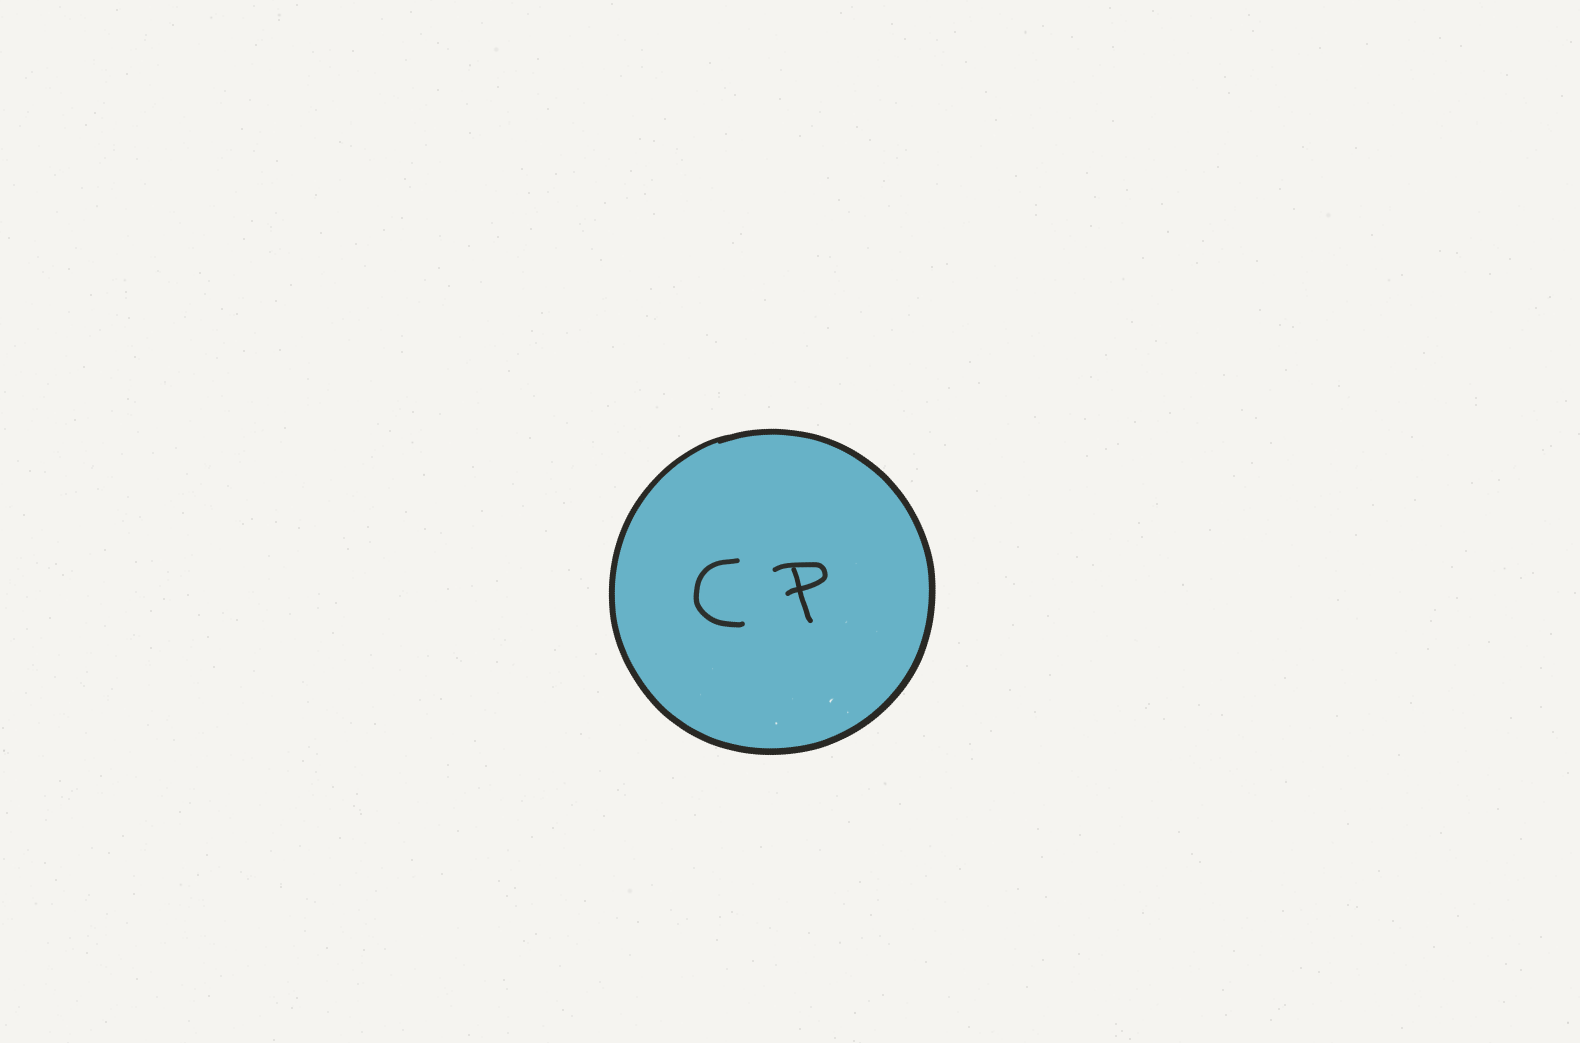
\includegraphics[height=2in]{figures/CP-cropped.png}\end{center}
    \onslide<3|handout:0>
    \begin{center}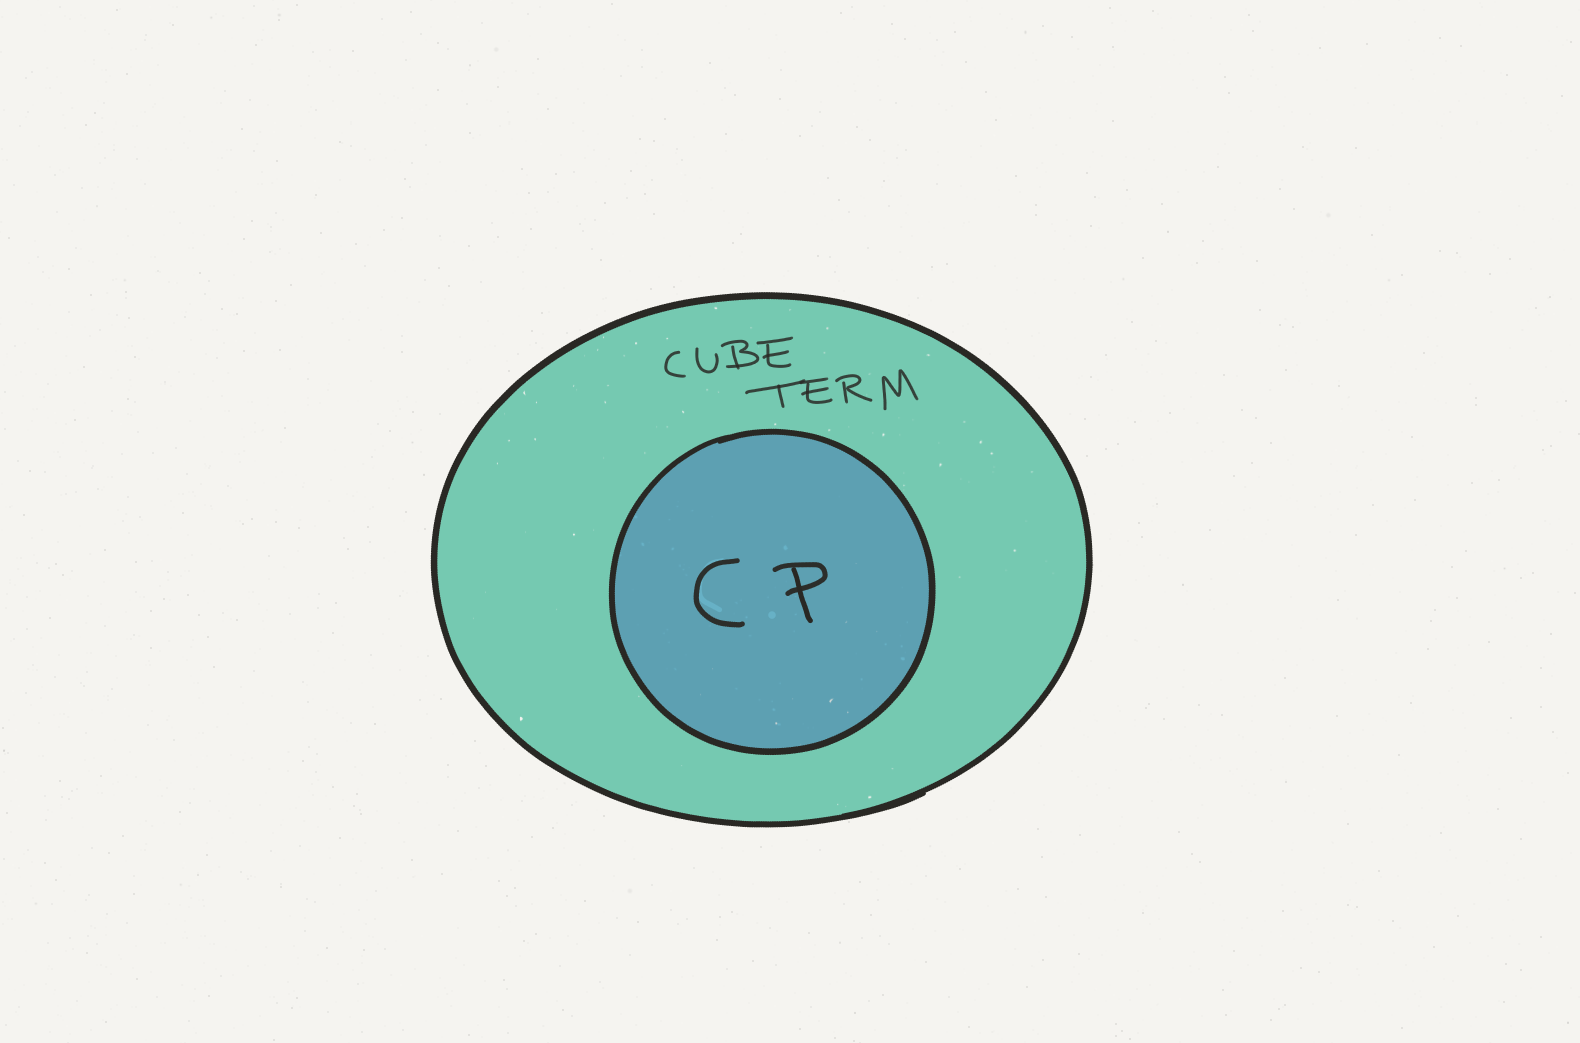
\includegraphics[height=2in]{figures/Cube-cropped.png}\end{center}
    \onslide<4|handout:0>
    \begin{center}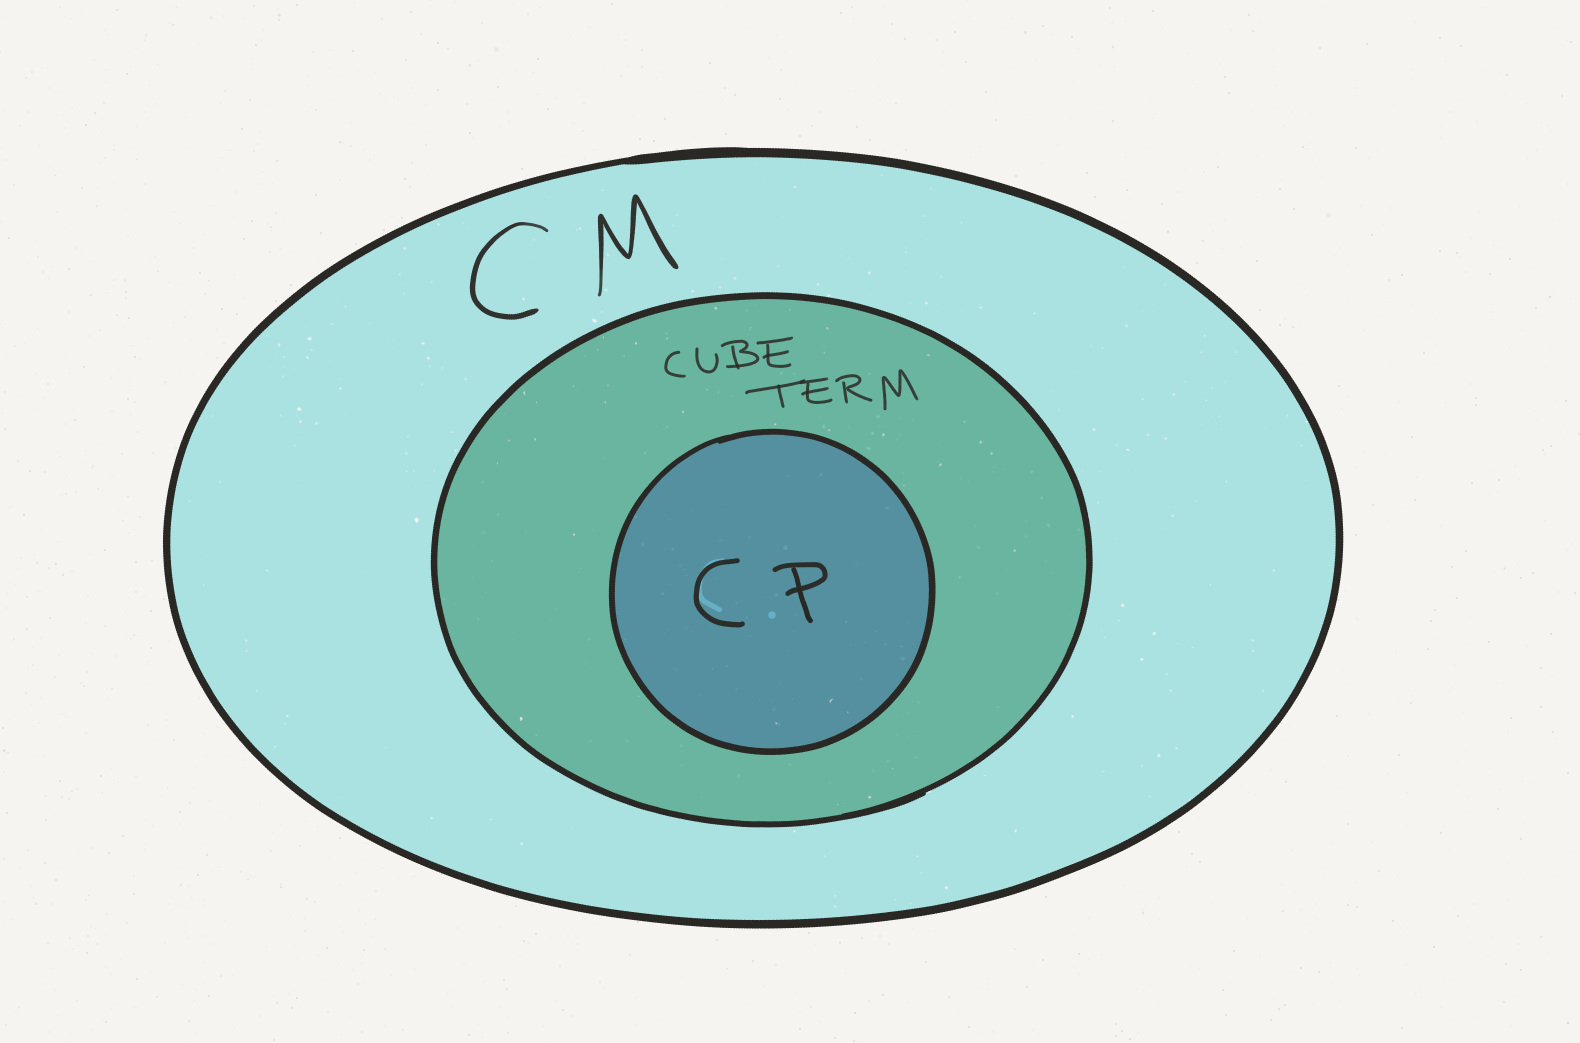
\includegraphics[height=2in]{figures/CM-cropped.png}\end{center}
    \onslide<5|handout:1>
    \begin{center}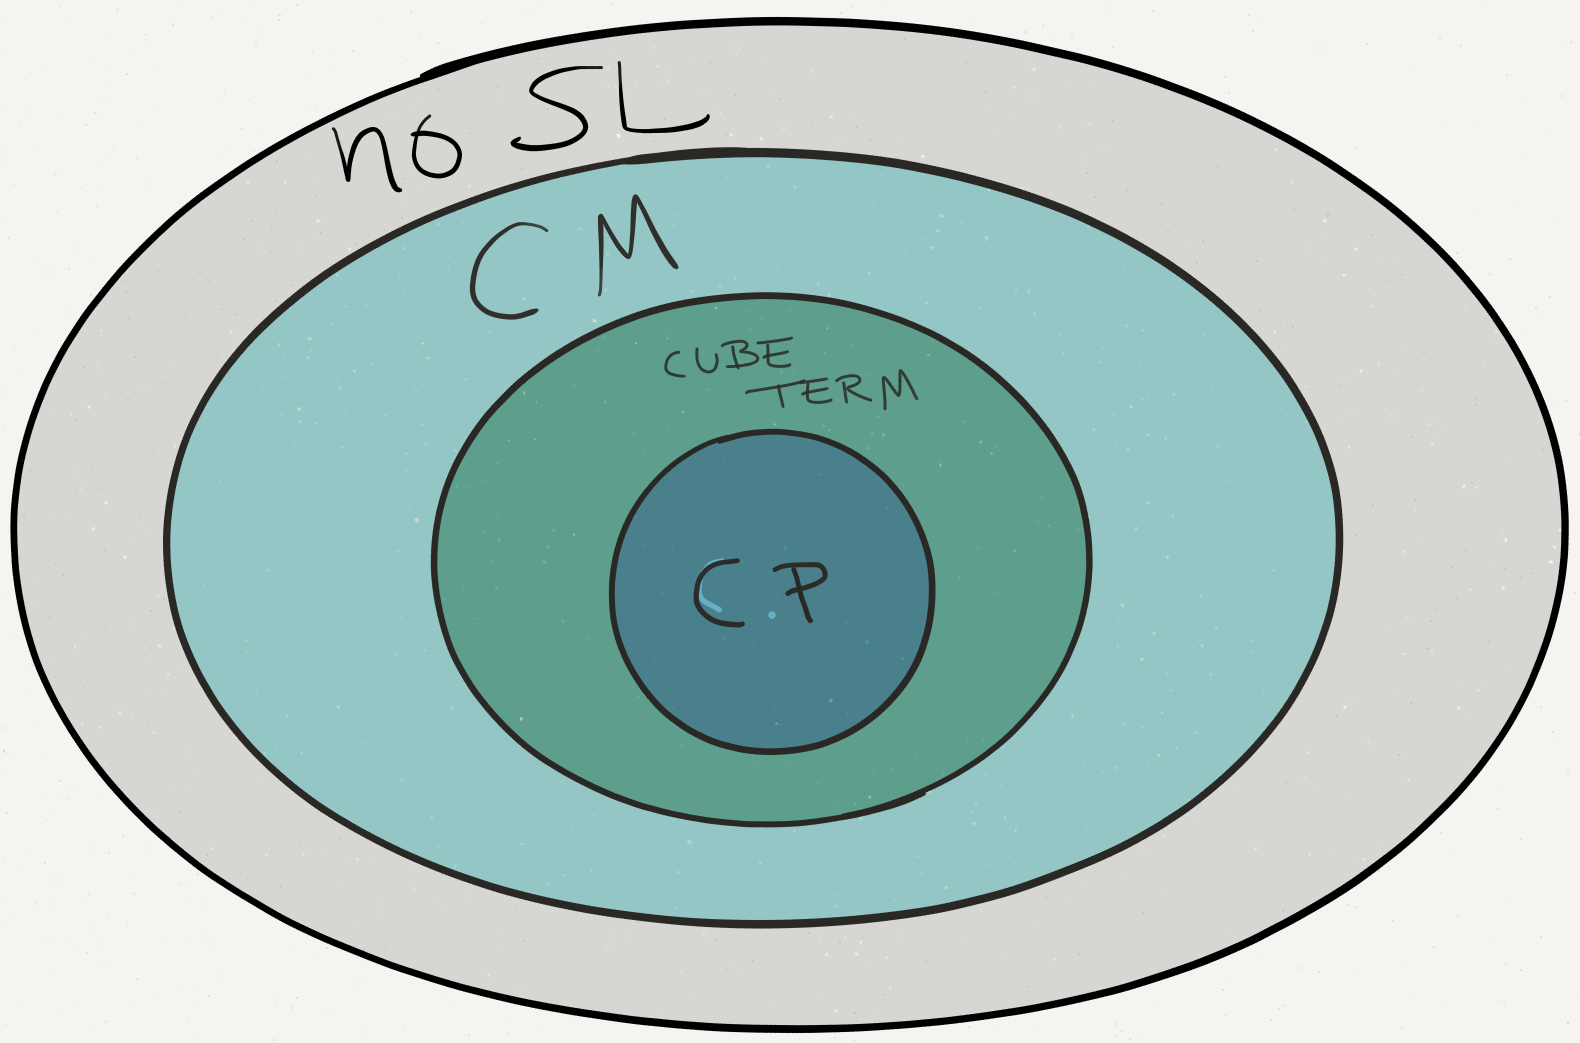
\includegraphics[height=2in]{figures/NoSL-cropped.png}\end{center}
  \end{overprint}
}




%%%%%%%%%%%%%%%%%%%%%%%%%%%%%%%%%%%%%%%%%%%%%%%%%%%%%%%%%%%
%% 10
\frame[label=cube]{
  \frametitle{First Reduction}
  \framesubtitle{by Cube-Term Blockers}

  Markovi{\'c}, M.~Mar{\'o}ti, McKenzie ($M^4$)\\
  ``Finitely related clones and algebras with cube terms'' (2012)

  \begin{block}{}
    %% \begin{definition}
    A \alert{cube-term blocker} (CTB) is a pair $(C, B)$ of subuniverses
    %% of $\bA$ 
    satisfying $\emptyset < C < B \leq A$ and for every
    $t(x_1, \dots, x_n)$ %% of $\bA$ 
    there is an index $i \in [n]$ with
    \[
    (\forall (b_1, \dots, b_n) \in B^n) (b_i \in C \longrightarrow t(b_1, \dots, b_n)\in C)
    \]
  \end{block}
    \onslide<2->
    \[
    t(b_1, \dots, b_{i-1}, c, b_{i+1}, \dots, b_n)\in C
    \]
  %% \end{definition}
  %% We call a set $D$ a (proper) \defn{ideal} of a \cib $\bA = \< A, \cdot\>$
  %%   if $D$ is a (proper) subset of $A$ satisfying $d\cdot a \in D$ for all 
  %% $d\in D$ and $a \in A$.
    \onslide<3->$M^4$ prove a finite idempotent algebra has
    a cube term iff it has no CTB.  

  \vfill
  \onslide<4->{
    \begin{lemma}
      A finite CIB $\bA$ has a CTB if and only if 
      $\bS_2 \in \sansH \sansS (\bA)$.
    \end{lemma}
    \onslide<5->{
      \begin{proof}
        $(C, B)$ a CTB implies
        $\theta = C^2 \cup (B- C)^2$ a congruence with $\bB/\theta \cong \bS_2$. 
        \\[5pt]
        Conversely, suppose $\bS_2 \in \sansH \sansS (\bA)$, and $\bB$ is 
        a subalgebra of $\bA$ with $\bB/\theta$ a meet-SL for some $\theta$. 
        Let $C/\theta$ be the bottom of $\bB/\theta$, then $(C, B)$ is a CTB.
      \end{proof}
    }
  }
}



%%%%%%%%%%%%%%%%%%%%%%%%%%%%%%%%%%%%%%%%%%%%%%%%%%%%%%%%%%%
%% 11
\frame[label=cp]{
  \frametitle{Second Reduction}

  Kearnes and Tschantz\\
  ``Automorphism groups of squares and of free algebras'' (2007)

  \begin{lemma}
    If $V$ is an idempotent variety that is not congruence permutable, then there
    are subuniverses $U$ and $W$ of $\bF := \bF_V\{x, y\}$ %% (the 2-generated free
    %% algebra)
    satisfying 
    \begin{enumerate}[1.]
    \item $x\in U \cap W$
    \item $y \in U^c \cap W^c$
    \item $(U \times F) \cup (F \times W) \leq \bF^2$
    \end{enumerate}
  \end{lemma}
  \onslide<2->{
    For CIB's, either $U$ or $W$ will be an ideal.\\[4pt]
    This implies a CTB and a semilattice.}
}


%%%%%%%%%%%%%%%%%%%%%%%%%%%%%%%%%%%%%%%%%%%%%%%%%%%%%%%%%%%
%% 12: Some well known facts
\frame[label=general2]{
  \frametitle{}

  $\bA=$ a finite CIB \hskip1cm
  $\mathbf S_2=$ the 2-elt semilattice.

  \begin{align*}
    \V(\bA) \text{ is CP } &\Longleftrightarrow \quad \bA \text{ has a Malcev term}\\
    &\Longrightarrow \quad \bA \text{ has a cube term}\\
    &\Longrightarrow \quad \V(\bA) \text{ is CM}\\
    &\Longrightarrow \quad \bS_2 \text{ is not in } \V(\bA)
    \uncover<2-|handout:2-3>{ \\   &{\mathbf \Longrightarrow} \quad \bA \text{ has a cube term} }
    \uncover<3-|handout:3>{ \\   &{\mathbf \Longrightarrow} \quad \V(\bA) \text{ is CP } }
  \end{align*}

  \begin{columns}
    \begin{column}{0.4\textwidth}
      \begin{overprint}
        \onslide<1|handout:1>
        \begin{center}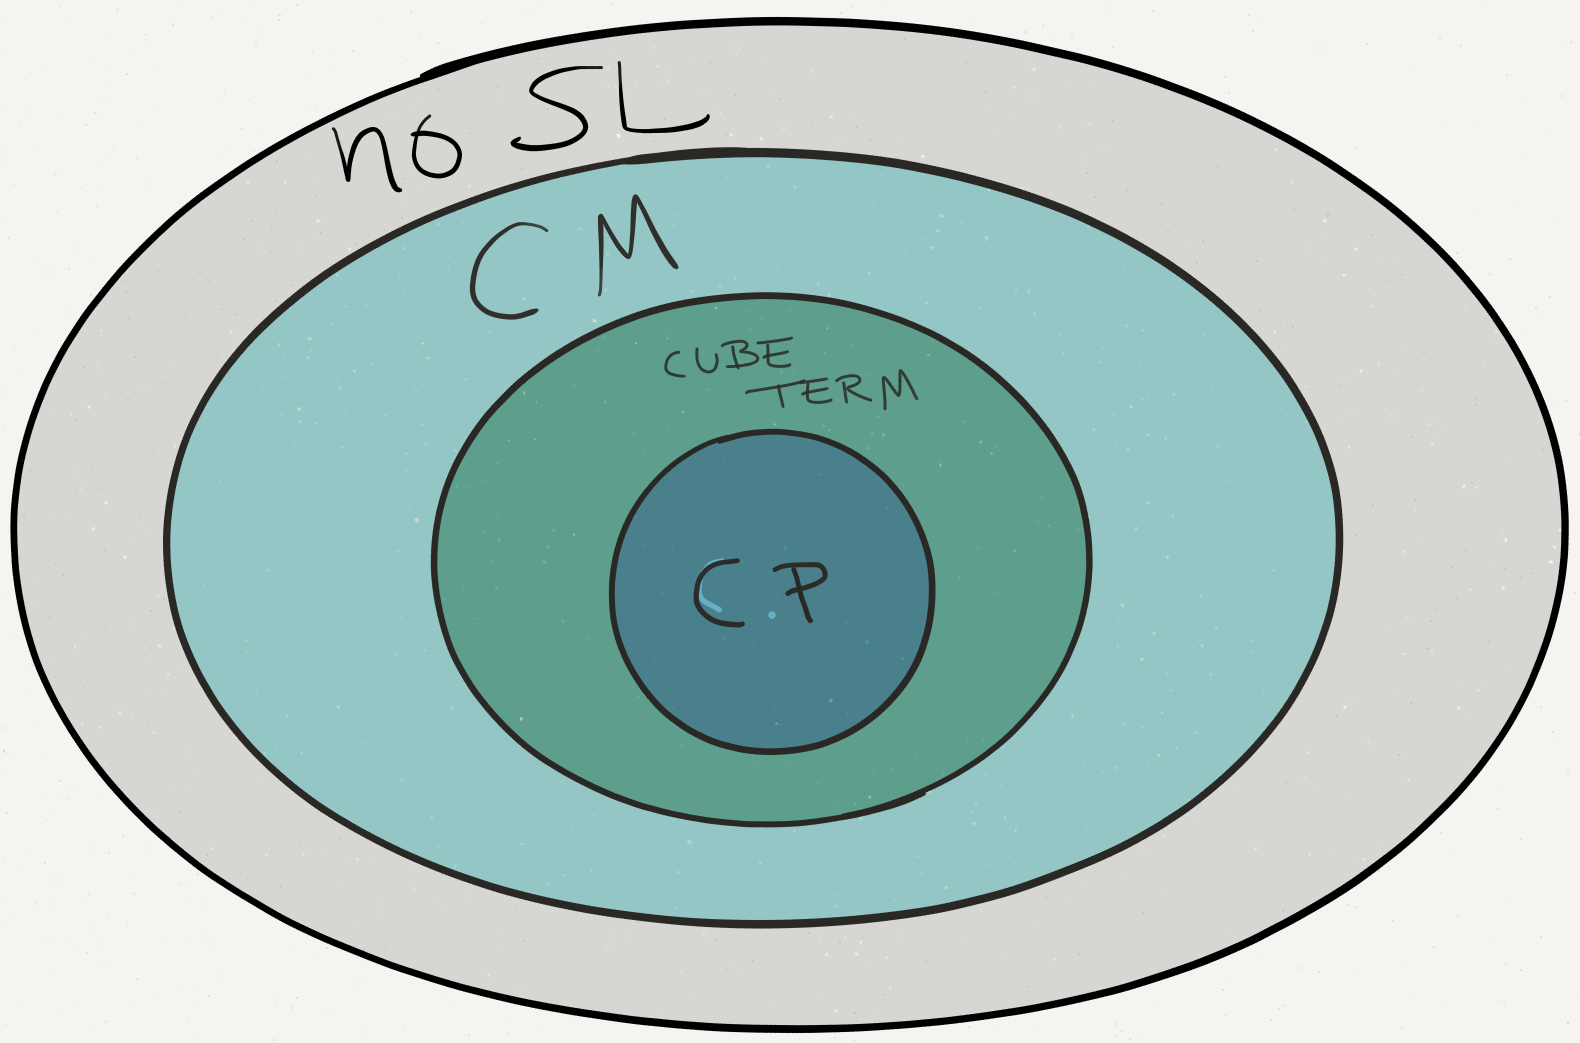
\includegraphics[height=1.25in]{figures/NoSL-cropped.png}\end{center}
        \onslide<2|handout:2>
        \begin{center}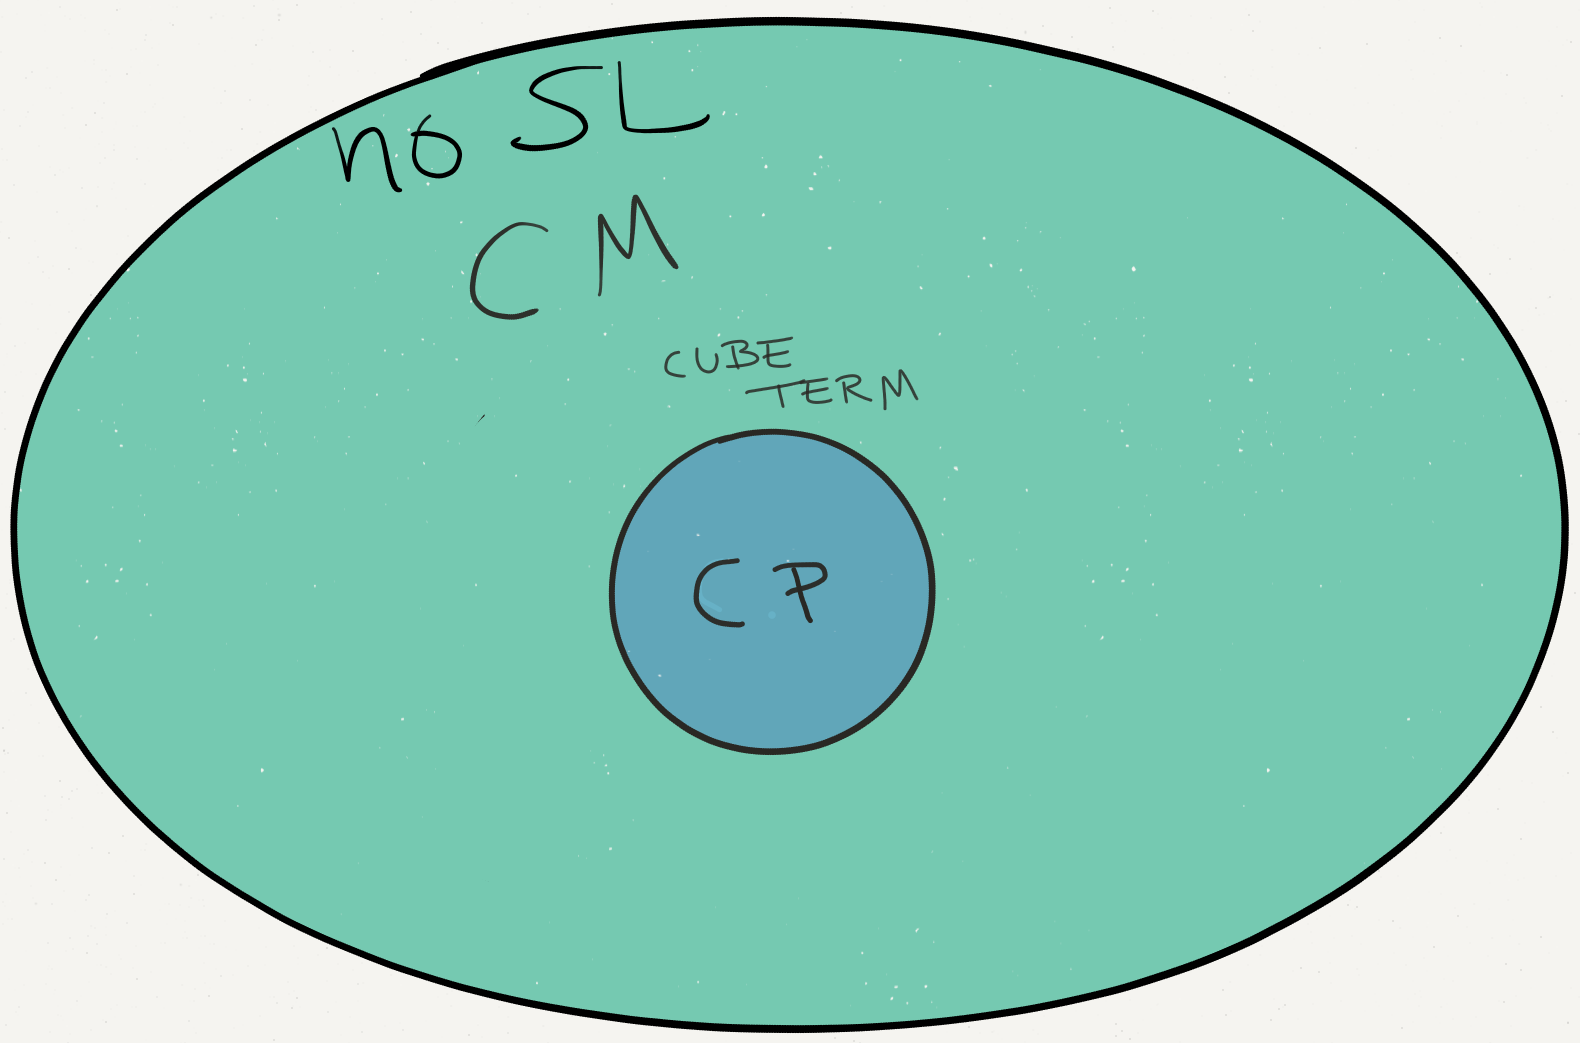
\includegraphics[height=1.25in]{figures/CubeEquiv-cropped.png}\end{center}
        \onslide<3|handout:3>
        \begin{center}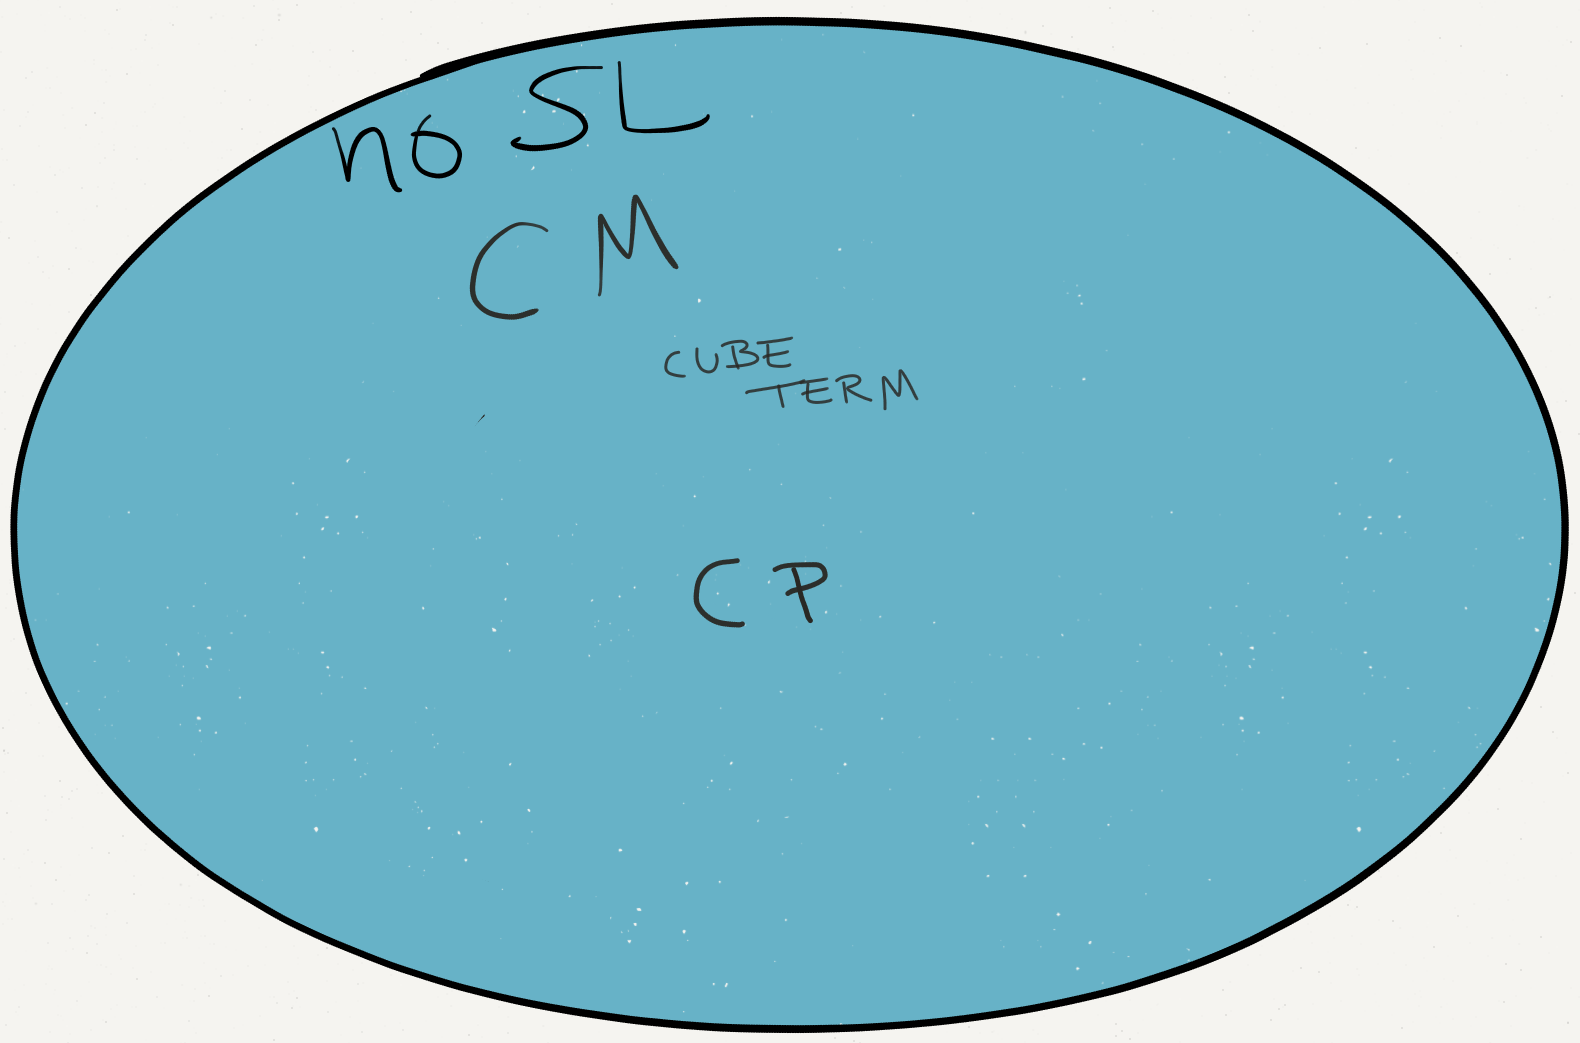
\includegraphics[height=1.25in]{figures/CPequiv-cropped.png}\end{center}
      \end{overprint}
      \vskip1cm
    \end{column}
    \begin{column}{0.6\textwidth}
        \begin{itemize}
        \item<2-|handout:2-3> 1st reduction by cube-term blockers.
        \end{itemize}
        \begin{itemize}
        \item<3-|handout:3> 2nd reduction by Kearnes-Tschantz.
        \end{itemize}
    \end{column}
  \end{columns}
}


%%%%%%%%%%%%%%%%%%%%%%%%%%%%%%%%%%%%%%%%%%%%%%%%%%%%%%%%%%%
%% 13
\frame[label=remaining]{
  \frametitle{Remaining Questions for Finite CIBs}

  \begin{block}{Conclusion}
    Let $\bA$ be a finite CIB. Then 
    \[
    \bS_2 \notin \sansH \sansS (\bA) \text{ if and
      only if } \V(\bA) \text{ is congruence permutable.}
    \]
    \onslide<2->(so $\CSP(\bA)$ tractable in this case)
  \end{block}

  \onslide<3->
  \begin{block}{Open Question}
    Let $\bA$ be a finite CIB with $\bS_2$ in $\sansH \sansS (\bA)$.  Is $\CSP(\bA)$ tractable?
  \end{block}

  \onslide<4->  Recall, 
  if $\V(\bA)$ is  $\mathrm{SD}_\wedge$, then $\CSP(\bA)$ is
  tractable.

  \onslide<5->
  \begin{block}{Revised Question}
    Let $\bA$ be a finite CIB with $\bS_2$ in $\sansH \sansS (\bA)$,
    and $\V(\bA)$ not $\mathrm{SD}_\wedge$.\\[4pt] 
    Is $\CSP(\bA)$ tractable?
  \end{block}

}

%%%%%%%%%%%%%%%%%%%%%%%%%%%%%%%%%%%%%%%%%%%%%%%%%%%%%%%%%%%
%% 14
\frame[label=examples1]{
  \frametitle{Example 1}

  \begin{columns}
    \begin{column}{0.4\textwidth}
  \begin{tabular}{c|cccc}
    $\cdot$ & 0 & 1 & 2 & 3\\
    \hline
    0 & 0 & 0 & 0 & 1\\
    1 & 0 & 1 & 3 & 2\\
    2 & 0 & 3 & 2 & 1\\
    3 & 1 & 2 & 1 & 3\\
  \end{tabular}
    \end{column}
    \begin{column}{0.6\textwidth}
      \onslide<2->
      \emph{Cliff's trick:} replace binary operation with a term from
      $\sansClo(\bA)$, say 
      \[x \ast y = (x\cdot(x\cdot y)) \cdot (y\cdot(x\cdot y))
      \]
      \\[6pt] 
      If $\<A, \ast\>$ tractable, then so is $\bA = \<A, \cdot\>$.
      \\[6pt] 
      \onslide<3->
      \begin{align*}
      \{\ast\} \subseteq \sansClo(\bA) \quad &\Longrightarrow \quad \sansRel(\sansClo(\bA)) 
      \subseteq \sansRel(\{\ast\})\\
      &\Longrightarrow \quad \CSP(\bA) \leq_P \CSP\<A, \ast\>
      \end{align*}
    \end{column}
  \end{columns}
  \onslide<4->
  \begin{columns}
    \begin{column}{0.4\textwidth}
      \begin{tabular}{c|cccc}
        $\ast$ & 0 & 1 & 2 & 3\\
        \hline
        0 & 0 & 0 & 0 & 0\\
        1 & 0 & 1 & 3 & 2\\
        2 & 0 & 3 & 2 & 1\\
        3 & 0 & 2 & 1 & 3\\
        \end{tabular}
    \end{column}
    \begin{column}{0.6\textwidth}
      $\<A, \ast\> \text{  tractable } \quad  \Longrightarrow \quad \bA 
\text{  tractable }$ 
    \end{column}
  \end{columns}
}



%%%%%%%%%%%%%%%%%%%%%%%%%%%%%%%%%%%%%%%%%%%%%%%%%%%%%%%%%%%
%% 15
\frame[label=examples2]{
  \frametitle{Example 2}

  \begin{columns}
    \begin{column}{0.4\textwidth}
  \begin{tabular}{c|cccc}
    $\cdot$ & 0 & 1 & 2 & 3\\
    \hline
    0 & 0 & 0 & 1 & 1\\
    1 & 0 & 1 & 3 & 2\\
    2 & 1 & 3 & 2 & 1\\
    3 & 1 & 2 & 1 & 3\\
  \end{tabular}
    \end{column}
    \begin{column}{0.6\textwidth}
      Let $t(x,y) = x\cdot(x\cdot(x\cdot y)) \cdot y\cdot (y\cdot(x\cdot y))$.
    \end{column}
  \end{columns}

\vskip3mm

  \onslide<2->
  \begin{columns}
    \begin{column}{0.4\textwidth}
      \begin{tabular}{c|cccc}
        $t$ & 0 & 1 & 2 & 3\\
        \hline
        0 & 0 & 0 & 0 & 1\\
        1 & 0 & 1 & 3 & 2\\
        2 & 0 & 3 & 2 & 1\\
        3 & 1 & 2 & 1 & 3\\
        \end{tabular}
    \end{column}
    \begin{column}{0.6\textwidth}
      $\<A, t\> \text{  tractable }$ 
    \end{column}
  \end{columns}
}

%%%%%%%%%%%%%%%%%%%%%%%%%%%%%%%%%%%%%%%%%%%%%%%%%%%%%%%%%%%
%% 16
\frame[label=examples3]{
  \frametitle{Example 3}

  \begin{columns}
    \begin{column}{0.4\textwidth}
  \begin{tabular}{c|cccc}
    $\cdot$ & 0 & 1 & 2 & 3\\
    \hline
    0 & 0 & 0 & 2 & 1\\
    1 & 0 & 1 & 3 & 2\\
    2 & 2 & 3 & 2 & 1\\
    3 & 1 & 2 & 1 & 3\\
  \end{tabular}
    \end{column}
    \begin{column}{0.6\textwidth}
\onslide<2->      Let $t_2(x,y) = \dots$ ?
\vskip2mm
\onslide<3->      Let $t_3(x,y,z) = \dots$ ?
    \end{column}
  \end{columns}
}
%%%%%%%%%%%%%%%%%%%%%%%%%%%%%%%%%%%%%%%%%%%%%%%%%%%%%%%%%%%
%% 17
\frame[label=others]{
  \frametitle{}
...and about 25 others.

\begin{center}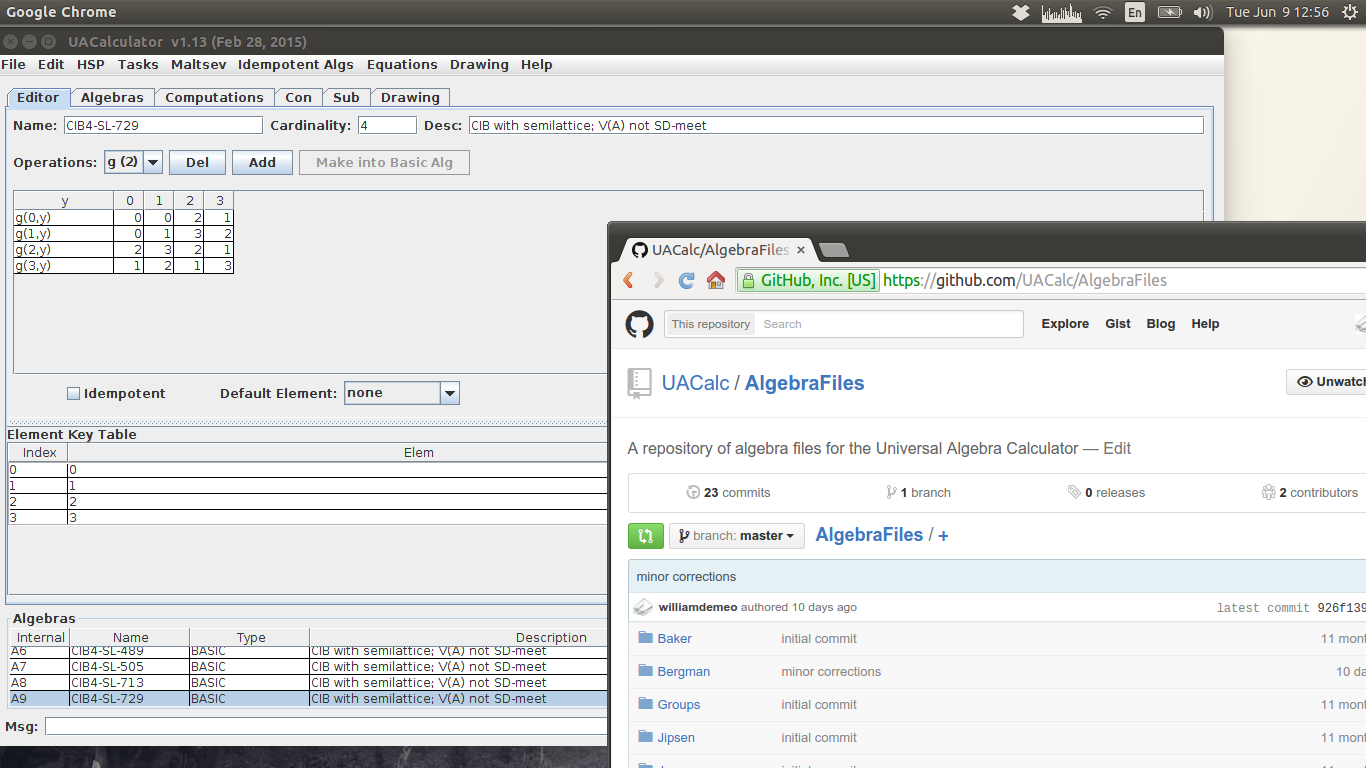
\includegraphics[height=2in]{figures/UACalcBergman.png}
%% \includegraphics[height=1.5in]{figures/BergmanDirectory.png}
\end{center}

To see them, load UACalc with files 
from the \alert{Bergman} directory at
\begin{center}
{\bf \url{https://github.com/UACalc/AlgebraFiles} }
\\[6pt]
\onslide<2->Thank you for listening!
\end{center}

}

\end{document}






Question: Does the converse of the last implication hold in general?
That is, if A is an finite idempotent algebra, then is it true that

S not in V(A)  =>  V(A) is CM?

This is certainly not true. For example, take A to be a 2-element set. However,
even if you omit type 1 it fails. Example 2.2 in the Freese-McKenzie paper on
Robust Maltsev conditions is an example. (It is actually an example due to
Matt.) You can probably find more examples by hunting through the Berman-Burris
catalog of 3-element binars:
http://www.math.uic.edu/~berman/1994-Groupoid-Catalog-Preprint.pdf 

It seems to me this is what Prop 3.9 and Cor 3.10 of Freese-Valeriote
says.  (If not, do you know a counter-example?)
No, the stuff about the tails is subtle. That's what Matt's example was designed to show.

I should know counter-examples for each of the converses that don't
hold.  Right now, I only know of one for "CM => cube term".  Namely,
the algebra Kearnes4.ua available here:

https://github.com/UACalc/AlgebraFiles/tree/master/Kearnes

has no cube term, but V(A) is CM.
This is the only example I am aware of.

What are examples of algebras with a cube term but no Malcev term.  (I
should know this! ...Jiali, feel free to jump in here!)
Every near-unanimity term is a cube term. So Lattices, for example, have cube terms but not Malcev terms. Also, the gmm terms of Dalmau are cube terms. I presume they are not always Malcev terms.

Now, back to the CIB case.  Once we prove (for CIBs) that

S not in V(A)  =>   V(A) is CP

then all the conditions above are equivalent.  That is,

For a finite CIB A, TFAE

1. V(A) is CP
2. A has a Malcev term
3. A has a cube term
4. V(A) is CM
5. S is not in V(A)
Correct. By the way, do we need A finite for this? I suspect not







